\section{Accurator framework}
\label{architecture}
To approach these challenges and evaluate our hypotheses, we develop the Accurator framework. We design the framework so that it allows us to easily test different strategies on various collections. Our main assumption is that making use of personalized nichesourcing increases the quality of annotations. We believe that we can automatically identify niche candidate users and create their user profiles. Based on the user profiles we can recommend relevant tasks to the user and apply trust mechanisms to improve the recommendations. Figure 1 shows the Accurator workflow. 

\begin{figure*}[hbt]
	\centering
	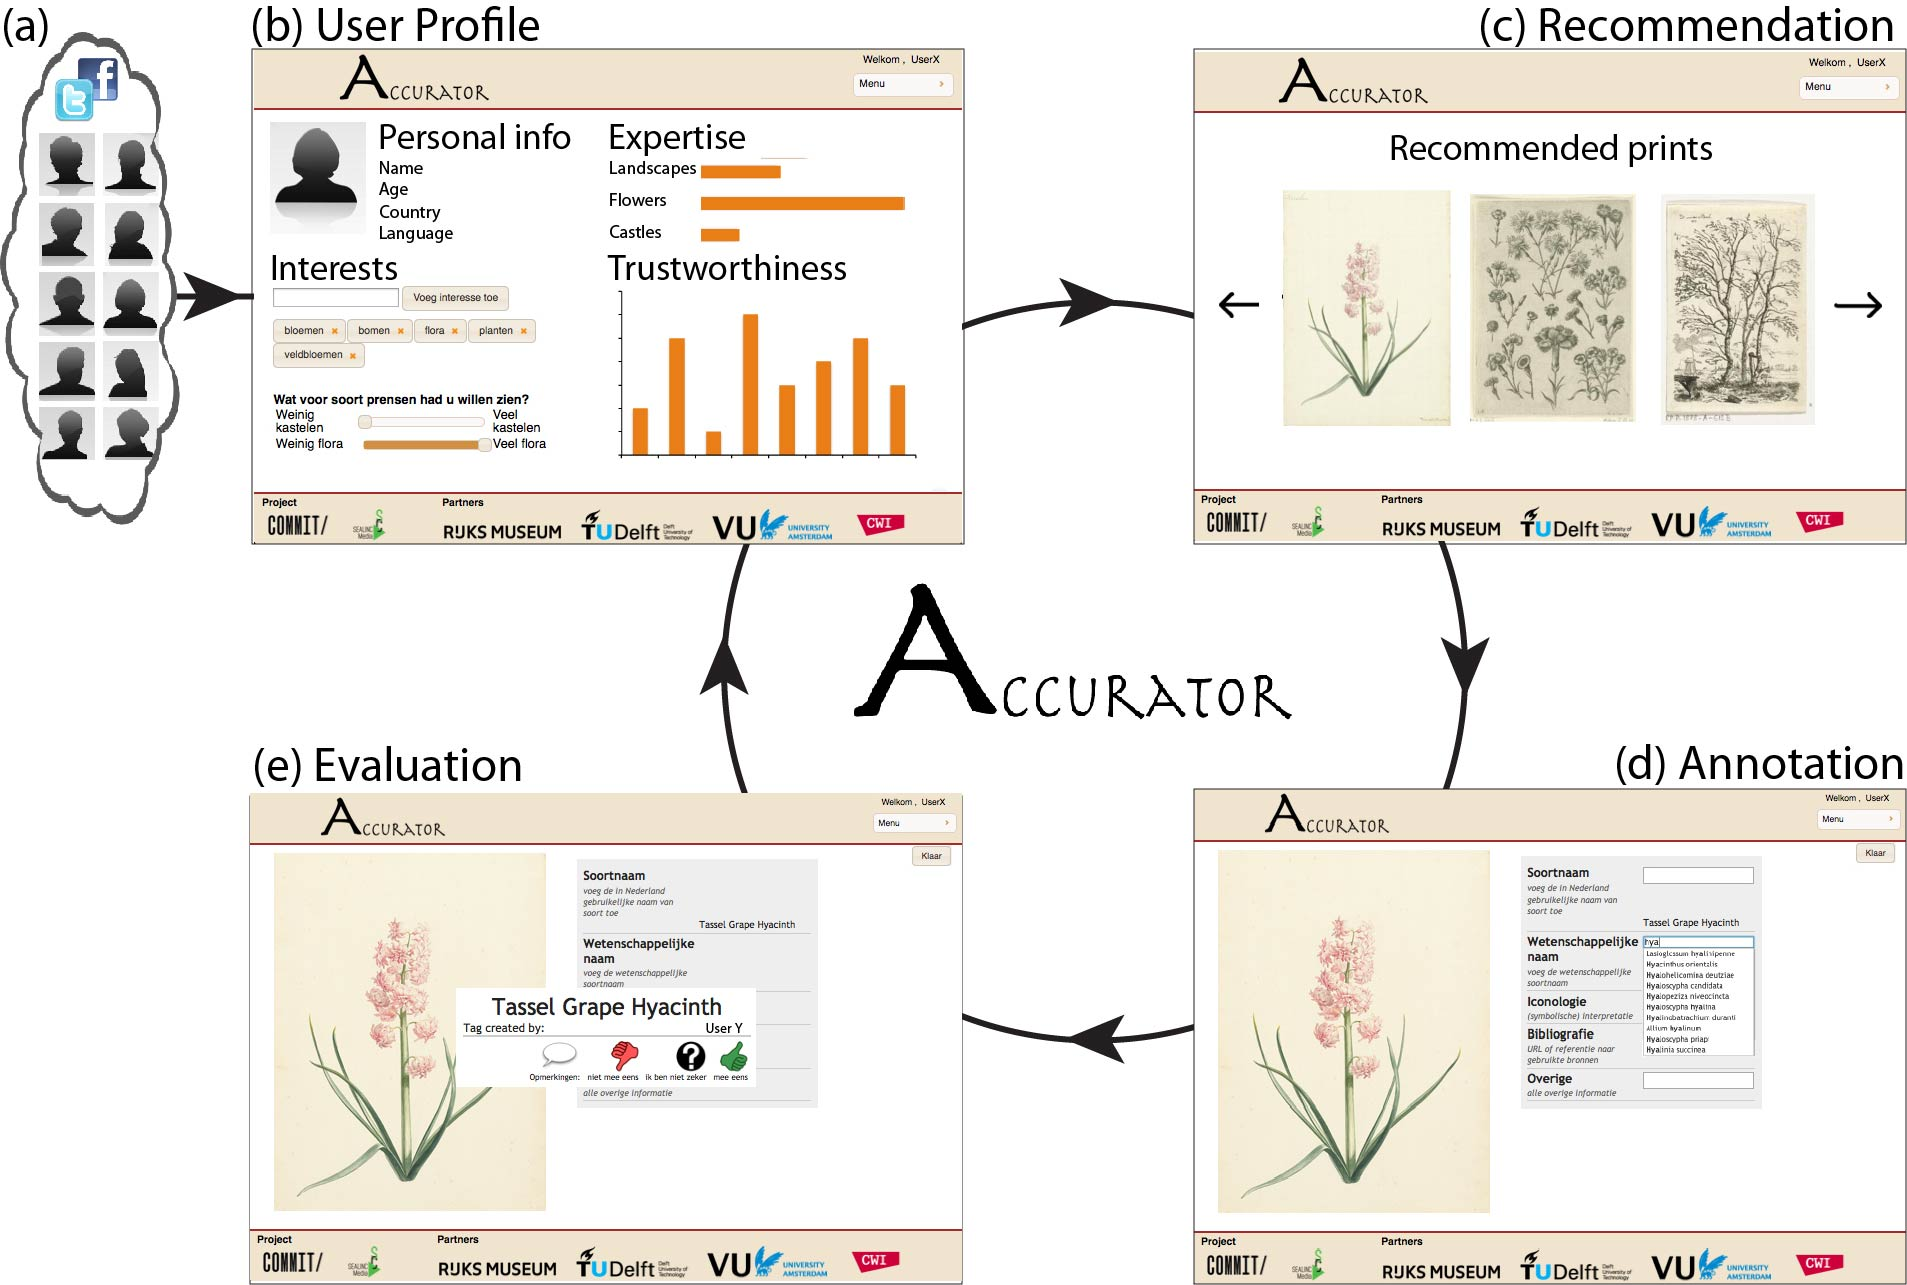
\includegraphics[width=0.93\textwidth]{accurator_diagram.jpg}
  	\caption{Accurator personalized nichesourcing workflow}
\end{figure*}

The process starts (see Figure 1a) with searching the social web for user-generated content that is relevant for a specific topic. We calculate the relevance of the content creators with respect to the topic and exploit social relations to identify a topical niche. When a person starts using Accurator, a user profile (see Figure 1b) is built based on available data.

Next (see Figure 1c) is the recommendation of collection items to a user. The recommendation strategy is based on specific patterns in the data, the user profile, and the current annotation quality of an item. Accurator allows to easily change between different strategies to cater for users diversity.
The choice of recommended items will affect the calculated interest of that user.

Figure 1d shows the interface where users add their annotations to an item. The presented fields depend on the topic and the user's expertise on that topic. 
Accurator can be configured to use domain vocabularies to support the user. Figure 1e shows the interface in which users can evaluate the annotations of other users. This task is only available to users who are trustworthy and have a certain level of expertise. The result of a review affects 1) the quality of an annotation, 2) the expertise level of the user and 3) the trustworthiness of another user.

The Accurator prototype is built using Cliopatria\footnote{\url{http://cliopatria.swi-prolog.org/}} to store RDF, Google Web Toolkit\footnote{\url{https://developers.google.com/web-toolkit/}} for the user interface and Google App Engine\footnote{\url{https://developers.google.com/appengine/}}  for hosting. Accurator is now used for experimentation with artwork data from the Rijksmuseum Amsterdam and a demo is available at 
\\ \url{http://rma-accurator.appspot.com}.



